\documentclass{beamer}
\usepackage[utf8]{inputenc}
\usepackage{graphicx}
\usepackage{xcolor}
\usepackage{listings}

\definecolor{commentgreen}{RGB}{2,112,10}
\definecolor{eminence}{RGB}{108,48,130}
\definecolor{weborange}{RGB}{255,165,0}
\definecolor{frenchplum}{RGB}{129,20,83}


\lstset {
    language=C++,
    frame=tb,
    tabsize=4,
    showstringspaces=false,
    numbers=left,
    %upquote=true,
    commentstyle=\color{commentgreen},
    keywordstyle=\color{eminence},
    %stringstyle=\color{red},
    basicstyle=\small\ttfamily, % basic font setting
    emph={int,char,double,float,unsigned,void,bool},
    emphstyle={\color{blue}},
    escapechar=\&,
    % keyword highlighting
    classoffset=1, % starting new class
    otherkeywords={>,<,.,;,-,!,=,~},
    morekeywords={>,<,.,;,-,!,=,~},
    keywordstyle=\color{weborange},
    classoffset=0,
}

\graphicspath{ {./images/} }

\title{Similarity Join}
\author{Filip Peterek}
\institute{VSB - Technical University of Ostrava}
\date{March 2022}

\begin{document}

    \frame{\titlepage}

    \begin{frame}
        \tableofcontents
    \end{frame}

    \section{Results}

    \begin{frame}
        \frametitle{Results}
        \begin{figure}
            \centering
            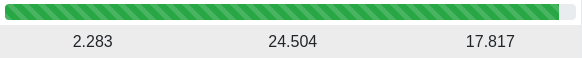
\includegraphics[width=0.9\textwidth]{images/pgcontest_time.png}
            \caption{Best result achieved by solution}
        \end{figure}
    \end{frame}

    \section{Iterations}

    \begin{frame}
        \frametitle{All-Pairs}
        \begin{itemize}
            \item All-Pairs algorithm
            \item Inverted Index
                \begin{itemize}
                    \item Separate index for each record size
                \end{itemize}
            \item robin\_hood::unordered\_flat\_map
        \end{itemize}
    \end{frame}

    \begin{frame}
        \frametitle{A Change of Utmost Importance}
        \begin{figure}
            \centering
            
\includegraphics[width=0.9\textwidth]{images/win_mentions.png}
            \caption{Most important improvement}
        \end{figure}
    \end{frame}

    \begin{frame}
        \frametitle{Parallelization}
        \begin{itemize}
            \item Two different approaches
                \begin{itemize}
                    \item Multiple queries in parallel
                    \item Parallel passes through multiple inverted indices
                    \item The latter proved to perform better
                \end{itemize}
            \item Parallel data loading
                \begin{itemize}
                    \item Open source blocking queue
                \end{itemize}
        \end{itemize}
    \end{frame}

    \begin{frame}
        \frametitle{Lower Level Optimizations}
        \begin{itemize}
            \item Fewer random accesses to memory
                \begin{itemize}
                    \item One index for a range of sizes
                    \item Index range depends on threshold
                \end{itemize}
            \item Fewer allocations
            \item Iterators over operator[]
        \end{itemize}
    \end{frame}

    \begin{frame}
        \frametitle{Index Size Ranges}
        \lstinputlisting[language=C++]{src/src.cpp}
    \end{frame}

    \section{Current State}

    \begin{frame}
        \frametitle{Current State}
        \begin{itemize}
            \item Index created before applying All-Pairs
                \begin{itemize}
                    \item Performance has been decreased slightly
                \end{itemize}
        \end{itemize}
    \end{frame}


\end{document}

